\section{Tính chất hai tiếp tuyến cắt nhau}
\thm{2 tiếp tuyến cắt nhau}{
	\textbf{Nếu 2 tiếp tuyến của một đường tròn cắt nhau tại một điểm:}\xd
	\textbullet Điểm đó cách đều hai tiếp điểm.\xd
	\textbullet Tia kẻ từ điểm đó đi qua tâm là tia phân giác của góc tạo bởi hai tiếp tuyến.\xd
	\textbullet Tia kẻ từ tâm đi qua điểm đó là tia phân giác của góc tạo bởi hai bán kính đi qua các tiếp điểm.
}

\begin{marginfigure}|-4.3cm|
	\centering
	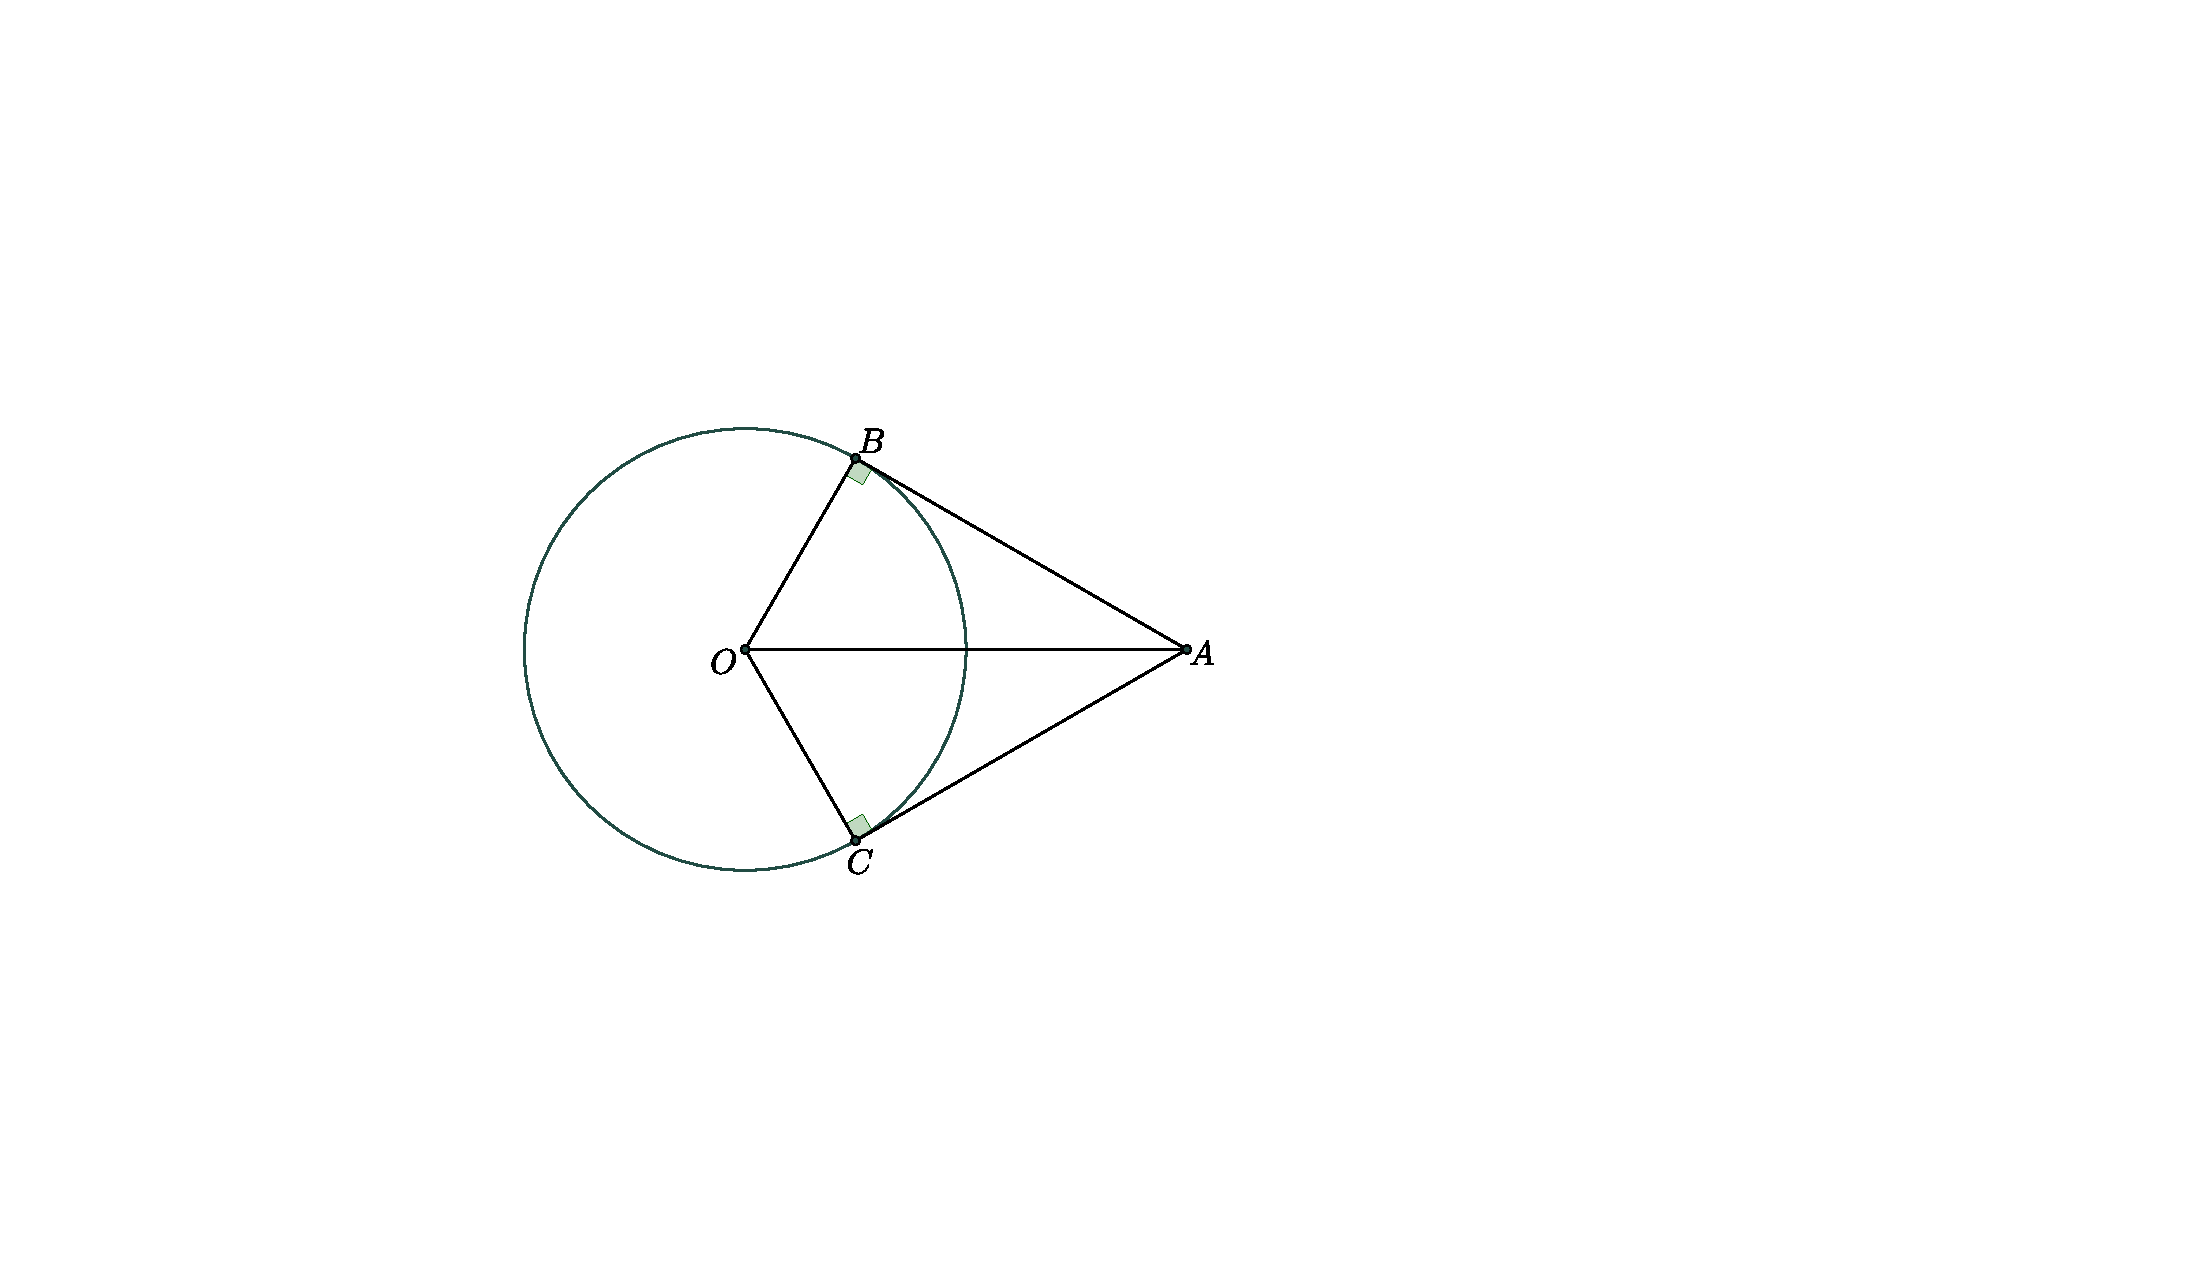
\includegraphics[width=0.9\marginparwidth]{img/tinh_chat_hai_tiep_tuyen_cat_nhau.pdf}
	\vspace{0.5cm}
	\margincaption{Tính chất hai tiếp tuyến cắt nhau}
	\label{hinh2.5}
\end{marginfigure}
\hq{
Ta có thể hiểu tính chất này một cách đơn giản như sau. Nếu 2 tiếp tuyến $AB$ và $AC$ cắt nhau tại $A$ \xd $\suyra$ 
$\begin{cases}
	AB = AC \xd
	\goc{BAO} = \goc{CAO} \xd
	\goc{BOA} = \goc{COA}
\end{cases}$ 
}{
\begin{center}
	Xét $\tamgiac AOB$ và $\tamgiac AOC $, có:\xd
$\begin{cases}
	AO \text{ là cạnh chung}\xd
	OB=OC~(=R)
\end{cases}$
\xd
$\suyra \tamgiac AOB = \tamgiac AOC~(ch-cgv)$\xd
$\suyra \begin{cases}
	AB = AC\xd
	\goc{BAO} = \goc{CAO}\xd
	\goc{BOA} = \goc{COA}
\end{cases}$
\end{center}
}

\begin{smallfont}
	\ex{Bài toán kinh điển}{
	Cho $(O; R)$ và 2 tiếp tuyến $AB; AC$ ($A$ nằm ngoài $(O; R)$)
	\begin{enumerate}[label=\alph*)]
		\item Chứng minh: $OA \vuong BC$.
		
		\item Gọi $H$ là giao điểm của $OA$ và $BC$. Chứng minh: $OB^2 = OH.OA$.
		
		\item Gọi $D \thuoc (O; R)$ ($D \khac B; C $). Chứng minh: $OD^2 = OH.OA$. 
	\end{enumerate}
	}
	
	\textbf{\textit{Lời giải:}}
		\begin{enumerate}[label=\alph*)]
			\item $\begin{cases}
				OB = OC = R \xd
				AB = AC ~(\textit{Tính chất 2 tiếp tuyến cắt nhau})
			\end{cases}$ \xd
			$\suyra$ $OA$ là đường trung trực của $BC$ \xd
			$\suyra$ \colorbox{themecolor!10!white}{$OA \vuong BC$}
			\item Xét $\tamgiac ABO$ và $\tamgiac BHO$, có: \xd
			$\begin{cases}
				\goc O \text{~chung} \xd
				\goc{ABO} = \goc{BHO} = 90^\circ
			\end{cases}$ \xd
			$\suyra \tamgiac ABO \dongdang \tamgiac BHO~(g-g)$ \xd
			$\suyra \frac{AB}{BH} = \frac{BO}{HO} = \frac{AO}{BO} \suyra \frac{BO}{HO} = \frac{AO}{BO}$ \xd
			$\suyra$ \colorbox{themecolor!10!white}{$OB^2 = OH.OA$}
			\item Có: $OD = OB = R$ \xd
			mà $OB^2 = OH.OA$ \xd
			$\suyra$ \colorbox{themecolor!10!white}{$OD^2 = OH.OA$} \qed
		\end{enumerate}
   
 	\begin{marginfigure}|-12cm|
		\centering
		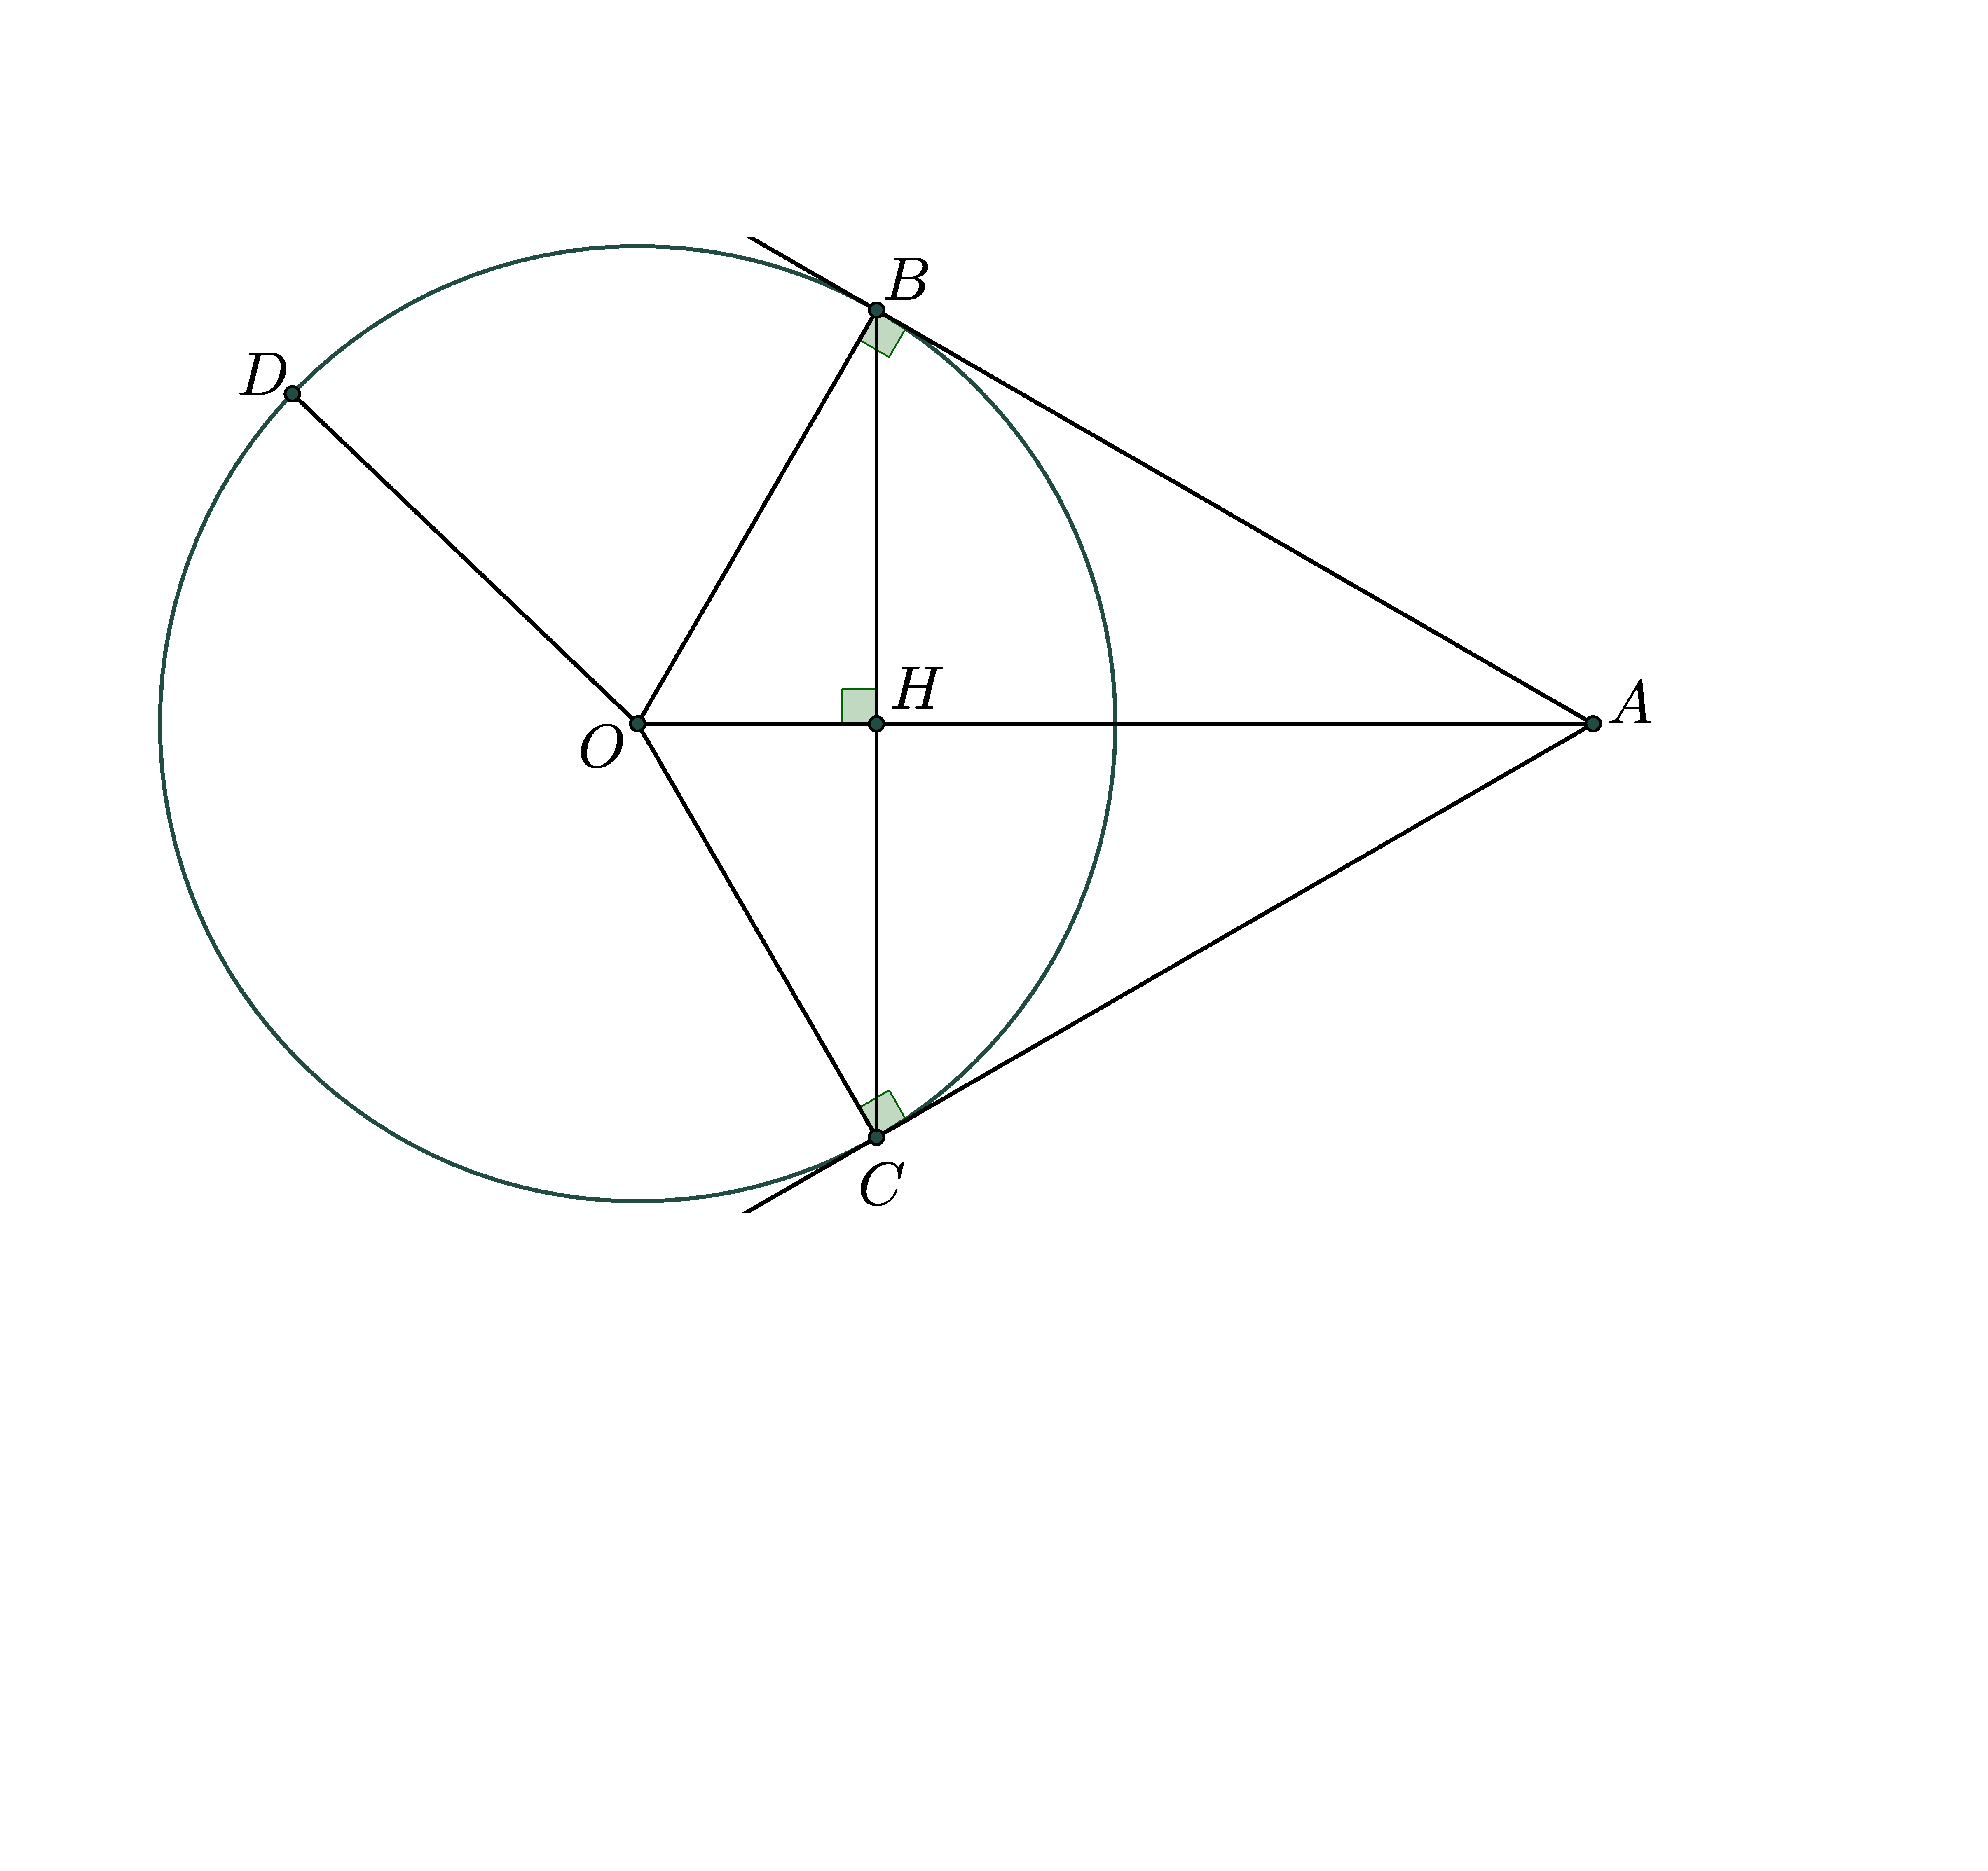
\includegraphics[width=0.8\marginparwidth]{img/vi_du_1.pdf}
		\vspace{0.5cm}
		\margincaption{Ví dụ 1}
		\label{hinh2.6c}
	\end{marginfigure}
\end{smallfont}
